\documentclass[tikz,border=2pt]{standalone}
\usepackage{amsmath}
\usetikzlibrary{arrows.meta}
\begin{document}
% Eigenvalues of the page's three examples against the unit circle |lambda| = 1:
% 0.5 (double; stable), 1.5 and -0.5 (unstable: 1.5 lies outside), 1 and 0.7 (boundary: 1 lies on the circle).
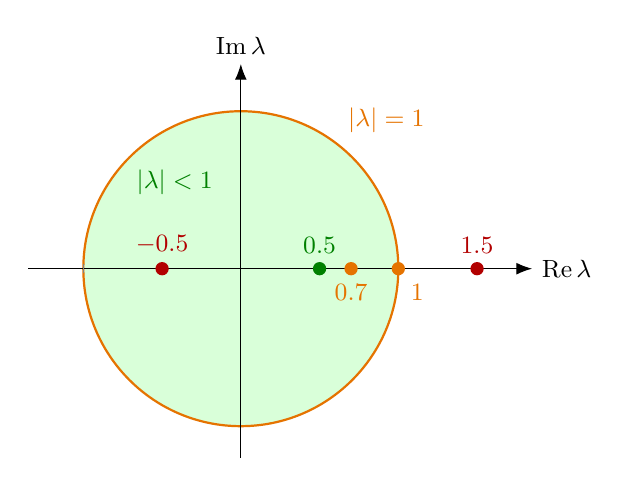
\begin{tikzpicture}[font=\small, >={Latex[length=2mm]}, x=2cm, y=2cm]
  \fill[green!15] (0,0) circle (1);
  \draw[orange!90!black, thick] (0,0) circle (1);
  \draw[->] (-1.35,0) -- (1.85,0) node[right] {$\operatorname{Re}\lambda$};
  \draw[->] (0,-1.2) -- (0,1.3) node[above] {$\operatorname{Im}\lambda$};
  \foreach \x in {-1,-0.5,0.5,1,1.5} \draw[gray] (\x,-0.03) -- (\x,0.03);
  \node[green!50!black] at (-0.42,0.55) {$\lvert\lambda\rvert<1$};
  \node[orange!90!black, anchor=south west] at (0.62,0.8) {$\lvert\lambda\rvert=1$};
  % example 1: only eigenvalue 0.5
  \fill[green!50!black] (0.5,0) circle (2.4pt) node[above, yshift=2pt] {$0.5$};
  % example 2: 1.5 and -0.5
  \fill[red!70!black] (1.5,0) circle (2.4pt) node[above, yshift=2pt] {$1.5$};
  \fill[red!70!black] (-0.5,0) circle (2.4pt) node[above, yshift=2pt] {$-0.5$};
  % example 3: 1 and 0.7
  \fill[orange!90!black] (0.7,0) circle (2.4pt) node[below, yshift=-2pt] {$0.7$};
  \fill[orange!90!black] (1,0) circle (2.4pt) node[below right, xshift=1pt, yshift=-2pt] {$1$};
\end{tikzpicture}
\end{document}
